\chapter{مبانی نظری}\label{chap3}
\minitoc

\section{مقدمه}

پس از تعریف مساله و مرور و بررسی روش‌های پیشنهاد شده توسط پژوهشگران، نوبت به ارائه راهکار پیشنهادی می‌رسد. البته راهکار پیشنهادی در این پژوهش خود بنا شده بر مدل‌های نوین ارائه شده در پردازش زبان است که نیازمند توضیح و بررسی می‌باشند.
از این رو، در این فصل مبانی نظری‌ای که پایه‌ها و ستون‌های راهکار پیشنهادی ارائه شده هستند، بیان و تشریح می‌شوند. در اولین بخش از این فصل معماری ترنسفورمر ارائه خواهد شد. در بخش دوم، شبکه‌های از پیش آموزش داده شده ترنسفورمری نظیر برت و بارت ارائه خواهند شد. آخرین بخش نیز به بررسی بعضی معیارهای سنجش تولید متن پرداخته شده است و یک معیار متفاوت از معیارهای مورد استفاده سایر پژوهش‌های مساله مکالمه، برای سنجیدن کیفیت پاسخ‌های تولید شده، ‌پیشنهاد می‌شود. 

\section{ترنسفورمرها}

تا قبل از پیدایش معماری ترنسفورمر غالب مدل‌های پردازش دنباله بر پایه‌ ساختار‌های پیچیده شبکه‌های بازگشتی و یا شبکه‌های 
\trans{پیچشی}{Convolutional}
بنا شده بودند و البته معمولا بهترین عملکرد این شبکه‌ها نیز در حالتی بود که شبکه‌های کدگذار و کدگشای خود را با مکانیزم توجه نیز به یکدیگر اتصال می‌دادند. 
مکانیزم توجه در واقع به قسمت کدگشا این اجازه را می‌دهد تا در هنگام تولید هر کلمه در رشته خروجی بتواند راحت‌تر وابستگی متناظر با آن کلمه را در رشته ورودی کشف و استفاده کند. در حالتی که مکانیزم توجه وجود نداشته باشد به علت کدشدن بازنمایی رشته ورودی در یک بردار با طول ثابت معمولا اطلاعات به سختی از قسمت کدگذار به کدگشا منتقل می‌شوند، حال آن که مکانیزم توجه با ایجاد اتصالات متعدد از کدگذار به کدگشا انتقال جریان اطلاعات از کدگذار به کدگشا و جریان مشتق از کدگشا به کدگذار را تسهیل کرده است.

ترنسفورمر
از نظر کارکردی در واقع یک مدل دنباله به دنباله کدگذار-کدگشا است که بدون استفاده از مکانیزم‌های بازگشتی صرفا بر مکانیزم توجه تکیه دارد
\cite{transformer}
. مدل‌های مبتنی بر ترنسفورمر اکنون پرچمدار
\trans{مرز دانش}{State of the Art}
بسیاری از زیرمسائل موجود در وظایف از جنس دنباله‌ای نظیر مدل‌زبانی
،
ترجمه ماشینی
، تشخیص موجودیت‌های اسمی، تحلیل احساسات
و بسیاری از زیرمسائل دیگر هستند.

ترنسفورمر به لحاظ ساختاری از دو زیرشبکه کدگذار و کدگشا تشکیل شده است.   
زیر شبکه کدگذار آن جمله مبدا را در ورودی گرفته و یک بازنمایی از آن را تولید میکند. زیر شبکه کدگشا نیز بازنمایی حاصل از زیر شبکه کدگذار و همچنین کلمات تولید شود تا حال حاضر از جمله مقصد را گرفته و سعی در تخمین توزیع احتمال کلمه بعد دارد. در شکل 
\ref{fig:chap3:transfoermer_overview}
نمایی کلی از معماری ترنسفورمر آورده شده است. در ادامه اجزای مختلف ترنسفورمر تشریح شده‌اند.


\begin{figure}[h]
	\centering
	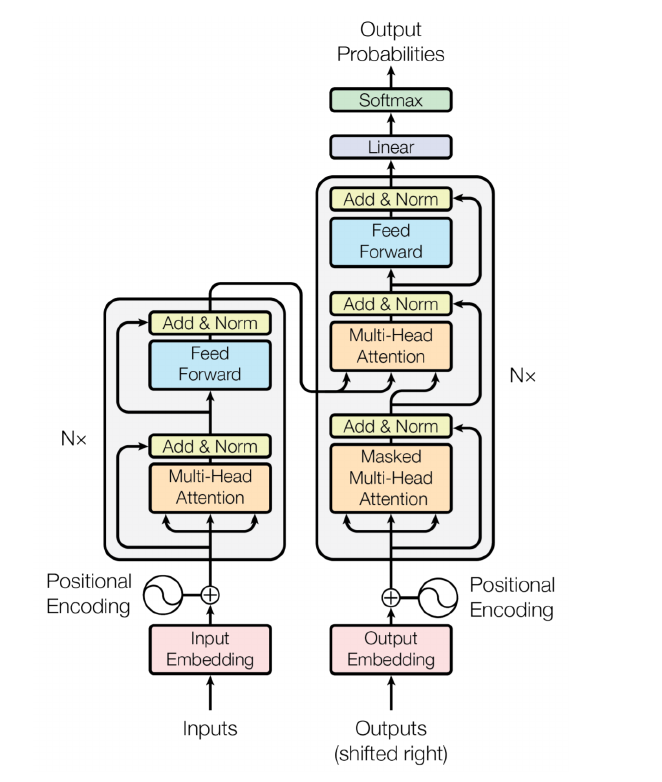
\includegraphics[width=0.85\textwidth]{images/chap3/transformer_arch.png}
	\caption[نمایی کلی از معماری ترنسفورمر]
	{
		نمایی کلی از معماری ترنسفورمر
		\cite{transformer}
	}
	\label{fig:chap3:transfoermer_overview}
\end{figure}

\subsection{کدگذار و کدگشا}
قسمت کدگذار ترنسفورمر از یک 
\trans{پشته}{Stack}
از چندین لایه یکسان تشکیل شده است که هر لایه خروجی خود را به عنوان ورودی به لایه بعدی تحویل می‌دهد. در هر لایه پشته کدگذار دو بلوک وجود دارد. بلوک اول یک مکانیزم 
\trans{خودتوجه چندسر}{Multi-Head Self-Attention}
است و بلوک دوم نیز یک شبکه عصبی 
\trans{پیشرو}{Feed-Forward}
\trans{تمام متصل}{Fully connected}
است که مستقل از مکان عمل می‌کند. در ضمن در هر بلوک نیز از 
\trans{اتصالات باقی‌مانده}{Residual Connection}
و 
\trans{هنجارساز لایه}{Layer Normalization}
استفاده می‌شود.

زیر شبکه کدگشای ترنسفورمر نیز مانند کدگذار دارای چندین لایه است با این تفاوت که هر لایه دارای سه بلوک است. بلوک اول و بلوک سوم کدگشا دقیقا مانند بلوک های اول و دوم کدگذار هستند. بلوک میانی اما در واقع نقش اتصال کدگذار و کدگشا را دارد و به وسیله یک توجه چند سر، مکانیزم توجه را روی خروجی آخرین لایه کدگذار انجام می‌دهد. در ضمن یک تفاوتی که در بلوک اول کدگذار با کدگشا وجود دارد این است که عمل توجه به خود در کدگشا صرفا بر روی ورودی‌های قبل از توکنی که قصد توجه دارد انجام می‌شود.


\subsection{مکانیزم توجه در ترنسفورمر}

\subsubsection{تعمیم مکانیزم توجه}
در این پژوهش مکانیزم توجه به شکل تعمیم یافته‌ای ارائه شده است. در واقع در مکانیزم توجه تعمیم یافته سه جزء اساسی بردار 
\trans{پرس و جو}{Query}
و یک جفت بردار‌های کلید-مقدار برای هر توکن در نظر گرفته می‌شوند. بردار خروجی مکانیزم توجه، حاصل جمع‌ وزن‌دار بردارهای مقدار  توکن‌های مورد توجه می‌باشد که این وزن‌ها خود تابعی از بردار 
پرس و جوی توکن در حال توجه و بردارهای کلید توکن‌های مورد توجه می‌باشند.

در روند پیاده‌سازی مکانیزم توجه در مدل ترنسفورمر از تابع ضرب داخلی به عنوان تابع محاسبه‌گر امتیاز مشابهت بردار‌های پرس و جو و کلید استفاده شده است.
سپس با اعمال تابع 
\trans{بیش‌نرم}{Softmax}
 روی تمامی امتیاز‌های مشابهت متعلق به توجه یک بردار پرس و جو بر روی مجموعه ای بردارهای کلید، وزن مربوطه ترکیب خطی مکانیزم توجه محاسبه می‌گردد. در نهایت از آن‌جایی که به ازای مقادیر بزرگ 
$d_k$
که اندازه بردار کلید است، حاصل ضرب داخلی بسیار بزرگ می‌شود و خروجی تابع 
بیش‌نرم
به گونه‌ای می‌شود که مشتق بسیار ضعیفی به عقب باز‌ می‌گردد، جهت رفع این مشکل، امتیازات قبل از اعمال 
بیش‌نرم
تقسیم بر 
$\sqrt{d_k}$
می‌شوند. جهت درک بهتر این عملیات شکل
\ref{fig:chap3:transformer_attention}
 آورده شده است.

\begin{figure}[h]
	\centering
	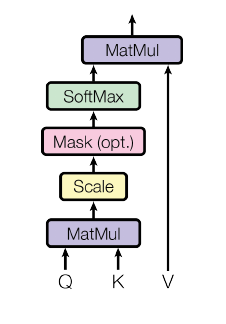
\includegraphics[width=0.3\textwidth]{images/chap3/transformer_attention.png}
	\caption[نمایی از مکانیزم نوجه در مدل ترنسفورمر]
	{
		نمایی از مکانیزم توجه در مدل ترنسفورمر
		\cite{transformer}
	}
	\label{fig:chap3:transformer_attention}
\end{figure}

\subsubsection{مکانیزم توجه چندسر}

نکته جالب توجه دیگر در معماری ترنسفورمر مکانیزم توجه چندسر است. در مقاله این گونه بیان شده که به جای این که هر بار یک توجه با ابعاد بردار 
$d_{model}$
انجام بگیرد، می‌توان بردارهای پرس و جو، کلید و مقدار را با کمک شبکه‌های پیشرو قابل یادگیری به تعداد
$h$
فضای با ابعاد
$d_{model/h}$
تصویر کرد و سپس 
$h$
عمل توجه را روی این بردار‌های تصویر شده انجام داد و در نهایت حاصل این توجهات را با یکدیگر الحاق کرد. مکانیزم توجه چندسر به مدل اجازه می‌دهد تا همزمان بتواند به اطلاعاتی از فضاهای 
\trans{بازنمایی}{representation}
مختلفی توجه کند. به علاوه امکان موازی‌سازی بین این عملیات‌های توجه نیز فراهم است و از این حیث مدل دچار هزینه زمانی اضافی نمی‌شود. برای درک بهتر مکانیزم توجه چندسر شکل 
\ref{fig:chap3:transformer_multihead}
آورده شده است.
\begin{figure}[h]
	\centering
	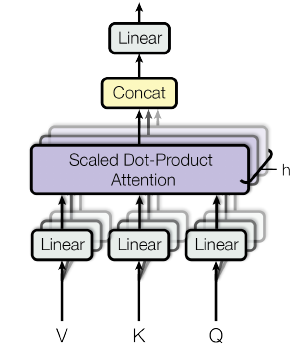
\includegraphics[width=0.4\textwidth]{images/chap3/transformer_multihead.png}
	\caption[نمایی از مکانیزم توجه چندسر در مدل ترنسفورمر]
	{
		نمایی از مکانیزم توجه چندسر در مدل ترنسفورمر
		\cite{transformer}
	}
	\label{fig:chap3:transformer_multihead}
\end{figure}


\subsubsection{موارد استفاده از توجه در ترنسفورمر}
مدل ترنسفورمر از مکانیزم توجه چندسر در سه موقعیت مختلف استفاده می‌کند:

\begin{itemize}
	\item 
	\textbf{توجه کدگشا به کدگذار}:
	در این بخش بردار‌های پرس و جو از لایه‌ی‌ قبلی کدگشا حاصل می‌شوند و بردارهای کلید و مقدار نیز از خروجی کدگذار به دست می‌آیند.
	
	\item 
	\textbf{توجه به خود کدگذار}:
	در این بخش تمامی بردارهای پرس و جو و کلید و مقدار از خروجی لایه قبلی کدگذار حاصل می‌شوند. هر توکن در هر مکانی در کدگشا می‌تواند به تمامی توکن‌ها (چه قبل و چه بعد از خود) توجه کند.
	
	\item
	\textbf{توجه به خود کدگشا}:
	این مورد مانند توجه به خود کدگشا است، با این تفاوت که هر توکن در کدگشا تنها می‌تواند به بردارهای مقدار و کلید توکن‌های قبل از خود توجه کند.
	
	
\end{itemize}

\subsection{شبکه پیشرو تمام متصل مستقل از مکان}
علاوه بر بلوک توجه، هر یک از لایه‌ها در کدگذار و کدگشا دارای یک بلوک شبکه عصبی تمام متصل پیشرو هستند. این شبکه به هر برداری در هر مکانی به صورت جدا و البته یکسان اعمال می‌شود (البته دقت شود که پارامتر‌های این شبکه‌های متصل لایه به لایه فرق می‌کنند). این شبکه یک شبکه با یک لایه مخفی است، اندازه بردارهای ورودی و خروجی آن ۵۱۲ می‌باشد و اندازه بردار حالت نهان آن هم ۲۰۴۸ است. کاربرد و فلسفه وجودی این شبکه در استخراج ویژگی از بردارهای حاصل از مکانیزم توجه است.


\subsection{
مکانیزم تعبیه
مکانی
}

از آنجایی که ساختار شبکه ترنسفورمر بازگشتی نمی‌باشد، بنابراین لازم است تا مکانیزمی جهت تزریق اطلاعات موقعیت مکانی کلمات دنباله نسبت به یکدیگر به مدل طراحی شود. به منظور حل این چالش در مدل ترنسفورمر برداری به نام بردار 
\trans{تعبیه}{Embedding}
 مکانی در نظر گرفته شده است که بنابر رابطه
\ref{eq:positional_embedding}
به دست می‌آید.

\begin{align} \label{eq:positional_embedding}
PE_{(pos, 2i)} = sin(pos/10000^{2i/d_{model}}) \\  \nonumber
PE_{(pos, 2i+1)} = cos(pos/10000^{2i/d_{model}}) 
\end{align}

این بردار تعبیه مکانی با اندازه 
\lr{$d_{model}$}
 به ازای هر توکن با مکان مختلف که متغیر
\lr{pos}
می‌باشد تعریف می‌شود. در نهایت بردار تعبیه مکانی با بردار تعبیه کلمه جمع خواهد شد.

\subsection{علت اهمیت به معماری ترنسفورمری}
ترنسفورمر‌ها به علت توانایی موازی‌سازی عملیات‌های خود در هنگام آموزش نسبت به شبکه‌های بازگشتی، سریعتر آموزش می‌بینند. از طرفی وجود عملیات توجه به خود چه در کدگذار و چه در کدگشا نیز خود عاملی برای تقویت این مدل نسبت به مدل‌های بازگشتی استفاده کننده از توجه شده است و به صورت خاص به نظر می‌رسد که وجود این توجه به خود برای مساله گفتگو بسیار موثرتر از وجود مکانیزم توجه بدون توجه به خود است.

\section{نهضت انتقال یادگیری در پردازش زبان}
تولد 
\trans{الگوواره}{paradigm}
 انتقال یادگیری را می‌توان مترادف با به وجود آمدن شبکه‌های غول آسایی نظیر
\LR{AlexNet}
و
\LR{VGG}
که بر روی دادگان عظیم تصویری آموزش یافته‌اند در نظر گرفت. محققان حوزه یادگیری عمیق و بینایی ماشین، با آموزش این مدل‌ها روی دادگان عظیم در پی این بودند که بتوانند بازنمایی‌های مناسبی از تصاویر به دست آورند؛ به نحوی که در روند حل مسائل دیگر بتوانند از آن‌ها به عنوان ویژگی‌ استفاده کنند. 

در حوزه متن اما اولین نمونه از انتقال یادگیری را می‌توان مدل معروف 
\lr{word2vec}
 ارائه شده توسط میکولوف در سال ۲۰۱۳ دانست
\cite{word2vec_paper}.
به این صورت که وظیفه حدس زدن کلمات اطراف یک کلمه توسط یک شبکه با یک لایه مخفی بر روی دادگان بسیار آموزش دیده شده و بازنمایی حاصل از آن شبکه به عنوان بازنمایی هر کلمه مدنظر قرار گرفت. پس از عرضه مدل 
\lr{word2vec}
مرز‌های دانش در بسیاری از مسائل پردازش زبان، بسیار فراتر از حد فعلی خود رفتند و این مدل کارایی خود را به نمایش گذاشت. اما از آن‌جایی که نقطه قوت این مدل از منظر انتقال یادگیری مورد توجه واقع نشد،‌ مسئله انتقال یادگیری نیز در حوزه پردازش زبان چند سال به خواب عمیقی فرو رفت تا آن که در سال ۲۰۱۸ مدل 
\lr{ELMO}
انتشار یافت
\cite{elmo_paper}.

توضیح آن‌که با وجود این که شبکه‌هایی نظیر 
\lr{word2vec}
برای هر کلمه یک بردار بازنمایی مناسب تولید می‌کردند اما وجود کلمات چند معنایی مانند "شیر" و یا "بستر" (که با آن که یک معنا دارد اما  در جمله‌ می‌تواند به معنای بستر خواب یا بستر رودخانه باشد) محققین را به این فکر انداخت که بازنمایی یک کلمه بایستی تابعی از محتوایی که آن کلمه در آن قرار گرفته نیز باشد.  به فرض مثال بازنمایی کلمه "شیر" در دو عبارت "من شیر را خوردم" و یا "شیر سلطان جنگل است" بایستی متفاوت بوده و تابعی از جمله باشد. 

به طور اجمالی مدل 
\lr{ELMO}
از دو شبکه 
\lr{LSTM}
چند لایه تشکیل شده است که یکی از آن‌ها وظیفه 
\trans{مدل زبانی}{Language Model}
را از سمت چپ و دیگری نیز وظیفه 
مدل زبانی
را از سمت راست روی دادگان متنی آموزش می‌بینند. 
\footnote{
توضیح آن که یادگیری وظیفه مدل زبانی از دو سمت باعث می‌شود تا بازنمایی بهتری برای کلمات به وجود بیاید. برای مثال دو عبارت "من شیر جنگل را دیدم" را با "من شیر را همراه با کیک میخورم" مقایسه کنید. در صورتی که تنها از یک شبکه بازگشتی استفاده کنیم و جمله را از راست به چپ به شبکه بازگشتی ورودی بدهیم بازنمایی کلمه شیر در هر دو عبارت یکی خواهد بود.
}
در مرحله بعد، در صورتی که بخواهند از این شبکه به عنوان نقطه شروع و یا شبکه استخراج ویژگی از کلمات برای یک وظیفه دیگر استفاده کنند، ترکیب خطی قابل یادگیری از بازنمایی کلمات در لایه‌های مختلف هر دو
\lr{LSTM}
را به عنوان بازنمایی آن کلمه در نظر می‌گیرند. برای درک بهتر معماری ELMO در شکل 
\ref{fig:chap3:elmo_arch}
به نمایش درآمده است.

\begin{figure}[h]
	\centering
	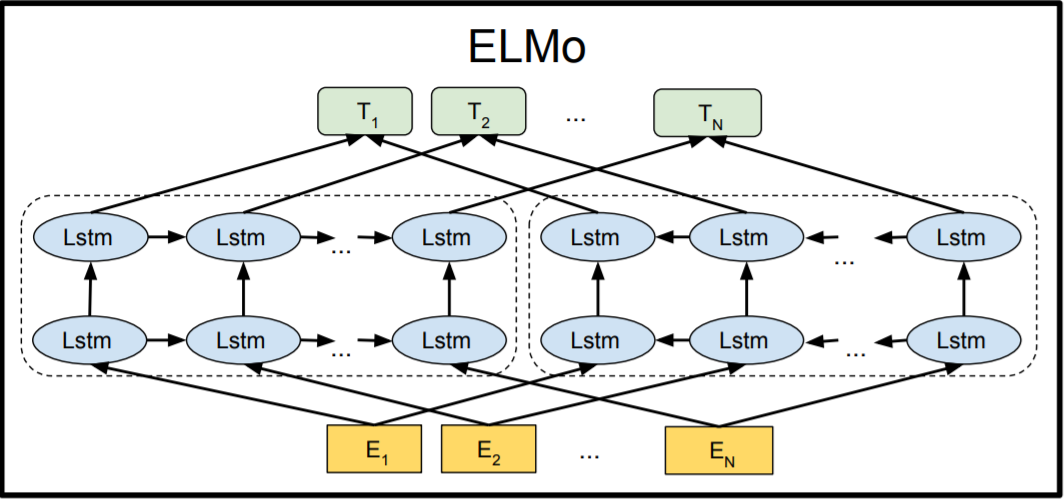
\includegraphics[width=0.8\textwidth]{images/chap3/elmo_arch.png}
	\caption{
		نمایی از معماری مدل المو
	}
	\label{fig:chap3:elmo_arch}
\end{figure}

 با ظهور مدل المو مرز‌های دانش در مسائل پردازش زبان گسترش پیدا کردند و امتیاز بهترین مدل‌ها در مسائل گوناگون پردازش زبان بهبود یافت. با این وجود به دلیل این که المو یک شبکه بازگشتی محسوب می‌شد، مشکلات شبکه‌های بازگشتی از قبیل توانایی کمتر در موازی‌سازی و همچنین انفجار یا ناپدید شدن گرادیان، در المو نیز وجود داشت.  

\subsection{مدل برت}
پس از ارائه معماری ترنسفورمر، توجهات در حوزه پردازش زبان از معماری‌های بازگشتی به معماری‌های ترنسفورمری معطوف گشت و در اغلب مسائل مهاجرت از معماری های بازگشتی به معماری‌‌ها نو شکل گرفت. 
طبعا این مهاجرت محققان این حوزه را نیز به این فکر انداخت تا مدلی با معماری ترنسفورمری و با کارکرد مشابه با المو ارائه دهند. سرانجام این ایده، منجر به انتشار مدل برت در سال ۲۰۱۹ گردید
\cite{bert}
.

مدل برت از لحاظ ساختاری، یک پشته کدگذار ترنسفورمری محسوب می‌شود. 
\footnote{در واقع ترنسفورمری است که تنها قسمت کدگذار را داراست و فاقد قسمت کدگشا است.}
هدف مدل برت مشابه المو به دست آوردن یک بازنمایی از طریق آموزش روی دادگان فراوان متنی بدون برچسب است. مزیت ساختاری برت بر المو را نیز می‌توان اولا در سرعت بالاتر و آموزش راحت شبکه‌ ترنسفورمری نسبت به شبکه بازگشتی دانست و از آن مهم‌تر امکان توجه توامان
\trans{دوطرفه}{Bidirectional}
 در هر کلمه نسبت به محتوای سمت چپ و راست آن دانست. در واقع در مدل برت بردار بازنمایی یک کلمه می‌تواند به کلمات سمت راست و چپ خود همزمان توجه کند در حالی که در مدل المو ما با دو شبکه بازگشتی مواجه هستیم که هر یک سعی دارند به طور غیرتوام توجه بردار بازنمایی کلمه را به سمت چپ و راست معطوف کنند. 
 
 در مقاله برت دو طرح اساسی مطرح شده است. طرح اول، چگونگی پیش آموزش شبکه برت و طرح دوم نیز چگونگی تنظیم آن روی وظایف مختلف پردازش زبان است.
 
 \subsubsection{چگونگی پیش‌آموزش برت}
 به منظور پیش آموزش شبکه برت، دو وظیفه 
 \trans{مدل زبانی پوشیده}{Masked-Language-Model}
 و 
 \trans{تشخیص جمله بعدی}{Next Sentence Prediction}
 انتخاب شده اند.
در مسئله مدل زبانی پوشیده، بر خلاف مسئله مدل زبانی عادی که در آن هدف یادگیری
\trans{توزیع احتمال}{Probability Distribution}
کلمه از روی کلمات قبلی‌اش است، هدف یادگیری توزیع اجتمال یک کلمه از روی کلمات قبل و بعد از خودش است. طبیعی است که با توجه به اهتمام برت بر به دست آوردن یک بازنمایی دوطرفه توامان وظیفه مدل زبانی پوشیده جهت نیل به این هدف بسیار موثر تر از وظیفه مدل زبانی عادی است. در هنگام پیش آموزش برت با وظیفه مدل زبانی پوشیده، به تصادف ۱۵ درصد از کلمات دنباله با توکن 
\lr{MASK}
تعویض می‌شوند و مدل بایستی بتواند که کلمه اول توکن‌های پوشیده شده را تشخیص دهد. 

با این که آموزش روی وظیفه مدل زبانی پوشیده به برت کمک می‌کند برای هر کلمه بازنمایی موثری بیابد اما برت برای انجام برخی مسائل پردازش زبان نیاز به ارائه بازنمایی مناسبی از جملات
و همچنین کشف رابطه بین جملات مختلف،
 نیز دارد. به این منظور، برت پس از پیش آموزش مدل زبانی پوشیده، روی وظیفه حدس جمله بعدی نیز آموزش می‌بیند. صورت این مساله این شکلی است که جمله A از دادگان آموزشی انتخاب می‌شود. سپس به احتمال پنجاه درصد جمله پس از A به عنوان جمله B انتخاب می‌شود و یا به احتمال باقی مانده پنجاه درصد یک جمله تصادفی به عنوان جمله B انتخاب می‌شود. سپس مدل بایستی این که آیا جمله B جمله بعدی جمله A است یا خیر را حدس بزند. 

 در پیاده‌سازی برت، هنگام ورود یک رشته در ابتدای آن یک توکن
\lr{[CLS]}
اضافه می‌شود که بردار بازنمایی حاصل آن از شبکه برت، بردار بازنمایی جمله را ارائه می‌دهد و در وظیفه تشخیص جمله بعدی، یک لایه
\lr{Softmax}
روی بردار بازنمایی
\lr{[CLS]}
اضافه گشته و احتمال خواسته شده را به دست می‌آورد. همچنین در پایان هر جمله نیز توکن
\lr{[SEP]}
اضافه می‌شود که جهت نشان دادن اتمام جمله ها به مدل به کار می‌رود. علاوه بر این، بردار
\trans{تعبیه قطعه‌ای}{Segment Embedding}
قابل یادگیری نیز با دو مقدار مختلف به دو جمله اول و دوم اعمال می‌شود. در واقع برت دارای سه مکانیزم تعبیه مکانی، قطعه‌ای و کلمه‌ای است که به ترتیب بر رشته ورودی اعمال می‌شود. جهت درک بهتر این تعبیه‌سازی‌ها، شکل
\ref{fig:chap3:bert_embeddings}
 آورده شده است.

 \begin{figure}[h]
 	\centering
 	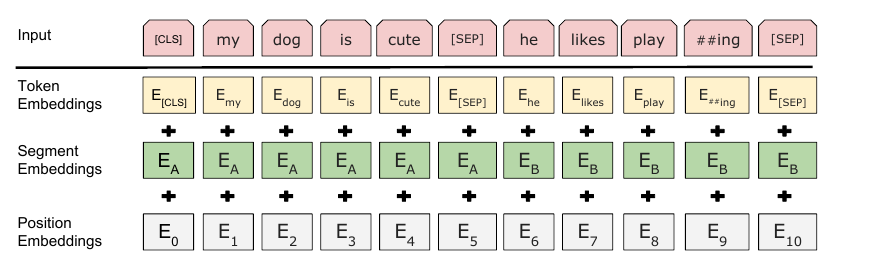
\includegraphics[width=1\textwidth]{images/chap3/bert_embeddings.png}
 	\caption[نمایی از انواع تعبیه در مدل برت]
 	{
 		نمایی از انواع تعبیه در مدل برت
 		\cite{bert}
 	}
 	\label{fig:chap3:bert_embeddings}
 \end{figure}

حسن و مزیت مسائل پیش آموزش برت در این است که دادگان بی‌برچسب موردنیاز آن‌ها به آسانی قابل جمع آوری است و همین باعث شده است که در طی دوره کوتاهی مدل برت 
توسط افراد مختلف
برای زبان‌های دیگر (از جمله فارسی) نیز آموزش یافته و در اختیار عموم قرار گیرد
\cite{parsbert}.

\subsubsection{نحوه تنظیم برت برای وظایف مختلف}
در مقاله برت،‌ پس از مشخص‌شدن نحوه پیش آموزش این شبکه، معماری‌های پیشنهادی مبتنی بر برت برای حل بعضی از مسائل پردازش زبان نظیر تحلیل احساسات، تشخیص موجودیت‌های اسمی و پرسش و پاسخ ارائه شده است. رویکرد حل این مسائل با برت به این نحو است که معمولا لایه‌هایی جهت حل مساله مورد نظر به برت پیش آموزش یافته اضافه می‌شوند و معماری جدید (که برت پیش‌آموزش یافته حالا جزیی از آن است) روی مساله مورد نظر و دادگان برچسب‌دار آن تنظیم می‌شود. 

\subsection{مدل‌های پس از برت}
با این که با عرضه برت، یک انقلاب در حوزه پردازش زبان و مسائلش رخ داد و مرز‌های دانش بسیاری از مسائل با استفاده از معماری‌های مبتنی بر برت پیشرفت قابل توجهی را تجربه کردند؛ اما برت بی عیب و نقص نیست و راه‌حل تمامی مسائل پردازش زبان نیز محسوب نمی‌شود. به دلیل ضعف‌های نسبی برت و همچنین موفقیت چشم‌گیر آن بسیاری از پژوهشگران نیز در ادامه کوشیدند تا شبکه‌های از پیش آموزش یافته دیگری که بر پایه معماری ترنسفورمر باشند، را پیش آموزش داده و عرضه کنند.
از مهم‌ترین این شبکه‌ها بایستی به سری شبکه‌های 
\lr{GPT}
اشاره کرد که با انتشار خود، باعث پیشروی مرز‌های دانش در حوزه مسائل تولید زبانی شدند و حتی با خروجی‌های شگفت انگیز خود همگان را حیرت زده کردند
\cite{gpt2_paper, gpt3_paper}.

و یا می‌توان به شبکه
\lr{Transformer-XL}
اشاره کرد که سعی دارد با اندکی تغییر در ساختار ترنسفومر، مشکل محدودیت برت 
(برت تنها می‌تواند متونی با حداکثر طول ۵۱۲ توکن را کد کند)
در طول متون ورودی را حل کند
\cite{DBLP:journals/corr/abs-1901-02860}.

با وجود همه این پیشرفت‌ها و حتی به راه افتادن رقابت بین شرکت‌های بزرگ دنیا بر سر آموزش دادن یک مدل بزرگتر و با تعداد پارامتر بیشتر، اما به نظر می‌رسد در طول این رشد و رقابت روزافزون بین مدل‌های از پیش آموزش یافته، غفلتی نسبت به بخشی از ایده اصلی ترنسفورمر‌ها صورت گرفته است. تمامی شبکه‌های از پیش آموز‌ش‌یافته ارائه شده تا قبل از مدل برت، را می‌توان تنها متشکل از یک پشته کدگذار معماری ترنسفورمر دانست. حتی تحت تاثیر این اتفاق، معماری‌های ارائه شده مبتنی بر این شبکه‌های از پیش آموزش یافته برای مسائل با ذات دنباله به دنباله نظیر مکالمه نیز، حالت دنباله به دنباله خود را از دست دادند و به صورت مدل زبانی مدل شدند
\cite{zhang2019dialogpt}.


\subsection{مدل بارت}
در حالی که بسیاری از محققین در حال صرف هزینه و تمرکز بر روی ایجاد مدل‌های تک پشته‌ای بودند، معماری دنباله به دنباله با عرضه مدل 
\trans{بارت}{Bart}
دوباره مورد توجه واقع شد. مدل بارت از لحاظ ساختاری یک ترنسفورمر کامل (پشته کدگذار به همراه پشته کدگشا) است. این مدل بر روی مساله بازسازی متن اصلی از روی متن 
\trans{خراب‌شده}{corrupted}
پیش آموزش می‌بیند و جهت بهینه‌سازی سعی در کمینه‌ کردن 
\trans{منفی لگاریتم بیشینه‌نمایی}{Negative Log Likelihood}
رشته خروجی می‌کند
\cite{lewis2019bart}.
 
 به صورت دقیق‌تر در طی فرآیند پیش‌‌‌ آموزش بارت، ابتدا داده‌‌ها (جملات) متنی بی برچسب توسط 
\trans{تابع نوفه‌ای‌ساز}{Noising Function}
دستکاری و به اصطلاح خراب می‌شوند. سپس این جملات خراب به مدل بارت ورودی داده می‌شود و بارت بایستی با استفاده از ساختار دنباله به دنباله خود، جمله اصلی را بازسازی کند. احتمال بازسازی جمله اصلی نیز از طریق محاسبه درست‌نمایی آن در کدگشای بارت حاصل می‌شود. برای درک بهتر این موضوع شکل
\ref{fig:chap3:bart_pretraining}
آورده شده است. در ضمن در هنگام تنظیم بارت روی وظایف دنباله به دنباله دیگر نظیر پرسش و پاسخ، متن پرسش به صورت سالم به قسمت کدگذار ورودی داده شده و از کدگشا انتظار می‌رود تا بتواند متن پاسخ را تولید کند.

 \begin{figure}[h]
	\centering
	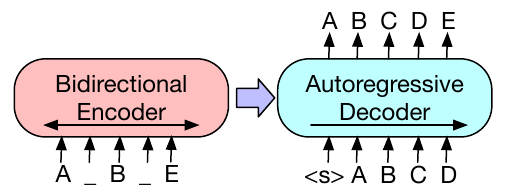
\includegraphics[width=0.6\textwidth]{images/chap3/bart_seq2seq.png}
	\caption[نمایی از نحوه پیش آموزش بارت]
	{
		نمایی از نحوه پیش آموزش بارت
		\cite{lewis2019bart}
	}
	\label{fig:chap3:bart_pretraining}
\end{figure}

ذکر این نکته ضروری است که بارت در پیش آموزش خود از پنج تابع آشوبگر زیر استفاده می‌کند:

\begin{itemize}
	\item 
	\textbf{
\trans{پوشاندن توکن‌ها}{Token Masking}	
}

به مانند مسئله پیش آموزش برت، در این جا نیز، توکن‌هایی به صورت تصادفی انتخاب شده و با نماد
\lr{\_}
جایگزین می‌شوند.

\item 
\textbf{
	\trans{حذف توکن‌ها}{Token Deletion}	
}

این تابع مانند مورد قبل است با این فرق که توکن انتخاب شده حذف می‌گردد و هیچ نمادی جای آن را نمی‌گیرد.

\item 
\textbf{
	\trans{پر یا خالی کردن متن}{Text Infilling}	
}

این تابع آشوبگر محدوده‌ای متن را انتخاب کرده (با طول توکن‌ دلخواه صفر، یک، دو و ...) سپس جای آن محدوده نماد 
\lr{\_}
را می‌گذارد.

\item 
\textbf{
	\trans{جایگردی جملات}{Sentence Permutation}	
} 

	این تابع آشوبگر متن را بر اساس علائم نگارشی خاتمه دهنده جمله نظیر نقطه، به دو قسمت تقسیم می‌کند و جای قسمت اول و دوم را عوض می‌کند.
\item 
\textbf{
	\trans{دوران متن}{Document Rotation}	
} 	

این تابع آشوبگر یک توکن را به تصادف انتخاب می‌کنند و متن را به گونه‌ای دوران می‌دهد که این توکن، آغازگر متن باشد.
\end{itemize}

جهت درک بهتر این توابع آشوبگر شکل
\ref{fig:chap3:bart_noising_function}
آورده شده است.
 \begin{figure}[h]
	\centering
	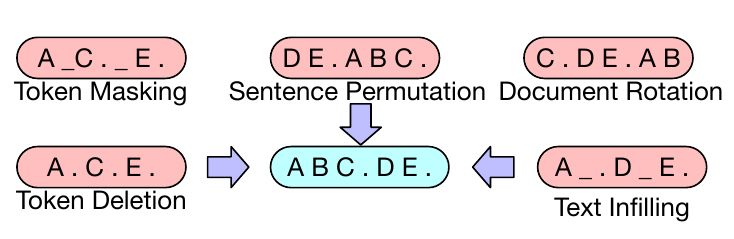
\includegraphics[width=0.6\textwidth]{images/chap3/bart_noising_function.png}
	\caption[نمایی از توابع نوفه‌ای‌ساز مورد استفاده در بارت]
	{
		نمایی از توابع نوفه‌ای‌ساز مورد استفاده در بارت
		\cite{lewis2019bart}
	}
	\label{fig:chap3:bart_noising_function}
\end{figure}

مدل بارت بر روی مسائل دنباله به دنیاله‌ای نظیر تنظیم ترجمه ماشینی و خلاصه‌سازی تنظیم شده و عملکرد موثری را ارائه داده است. به طوری که بهترین مدل‌های خلاصه‌سازی تا به اکنون، مدل‌های مبتنی بر بارت هستند. 

\section{شگرد عصاره‌گیری دانش 
}
ظهور شبکه‌ها و مدل‌های از پیش آموزش دیده با مقیاس بزرگ، با آن که پیشرفت قابل توجهی را در مسائل مختلف پردازش زبان رقم زدند؛ اما استفاده از آنان برای پژوهشگران چندان ساده نبود.
مقیاس بالا این شبکه و داشتن تعداد پارامتر‌های زیاد (از چند صد میلیون تا چند ده میلیارد حتی) مانع از استفاده موثر از آنان چه در زمان آموزش و تنظیم بر روی یک وظیفه و چه در زمان 
\trans{استقرار}{Deployment}
در جایگاه کاربردی می‌شود. در واقع تعامل با این مدل‌ها مستلزم در اختیار داشتن سخت‌افزار‌های پیشرفته است. در هنگام آموزش ورودی دادن یک
\trans{دسته}{batch}
از دادگان به این شبکه‌ها و خروجی گرفتن از آن‌ها مستلزم داشتن سخت‌افزار‌های با حافظه انبوه است و در هنگام استقرار به علت نیاز به پاسخ‌گیری 
\trans{بی‌درنگ}{Real-Time}
بایستی سخت‌افزاری فراهم بشود که بتواند با قدرت محاسباتی بالای خود به سرعت دادگان ورودی را از چند صدلایه سلول‌های عصبی عبور داده و خروجی را تولید نماید. 

در این هنگام بود که توجه پژوهشگران به ایده عصاره‌گیری دانش
که در سال ۲۰۱۵ ارائه یافته بود، معطوف شد
\cite{hinton2015distilling}.
عصاره گیری دانش شگرد فشرده‌سازی است که در آن یک مدل کوچک‌تر (که مدل دانش‌آموز نامیده می‌شود) آموزش می‌بیند تا رفتار مدل‌بزرگ‌تر (که مدل معلم نامیده‌می‌شود) را تقلید و بازتولید کند
\cite{hinton2015distilling}.

در فرآیند یادگیری بانظارت، مدل معمولا به گونه‌ای آموزش می‌بیند که بتواند توزیع احتمالاتی خود در مورد برچسب نمونه‌ها را به توزیع 
\trans{تک داغ}{One-Hot}
برچسب‌ آن‌ها نزدیک کند. این مهم معمولا از طریق کمینه‌سازی تابع هزینه
\trans{انتروپی متقاطع}{Cross-Entropy}
صورت می‌گیرد. جهت یادآوری آنتروپی متقاطع رابطه
\ref{eq:cross_entropy}
 آورده شده است که در آن $o$ بردار احتمالاتی تخمین زده شده توسط شبکه عصبی و $y$ نیز بردارتک فعال برچسب داده مورد نظر است.


\begin{align} \label{eq:cross_entropy}
L(y, o) = \sum_{i}^{} y_i\:log\,o_i
\end{align}

اما در فرآیند عصاره‌گیری، به طور اجمالی مدل دانش آموز از طریق کمینه‌کردن تابع هزینه عصاره‌گیری روی بردار‌های احتمالاتی خروجی مدل معلم آموزش می‌بیند. رابطه این تابع هزینه در رابطه
\ref{eq:cross_distill}

آورده شده است. در این رابطه $t$ بردار احتمالاتی حدس زده شده توسط مدل معلم و $s$ نیز بردار احتمالاتی حدس زده شده توسط مدل دانش آموز است.

\begin{align} \label{eq:cross_distill}
L_{ce} = \sum_{i}^{} t_i\:log\,s_i
\end{align}

اولین تلاش جدی در زمینه عصاره‌گیری از مدل‌های زبانی از پیش آموزش دیده را می‌توان مدل 
\lr{DistilBert}
دانست
\cite{sanh2019distilbert}.
این مدل سعی کرده است دانش مدل برت را 
تا حد ممکن به یک مدل با ساختار معماری مشابه برت ولی تعداد  لایه‌ها و پارامتر‌های کمتر انتقال دهد. در نهایت این مدل کوچکتر با تعداد پارامتر معادل ۶۰ درصد تعداد پارامتر‌های مدل برت اصلی،
توانسته به طرز حیرت آوری حدود ۹۷ درصد از عملکرد برت را روی وظایف مختلف حفظ کند. 

در ادامه در پژوهش دیگری، مدل‌های عصاره‌گرفته‌شده دیگری از برت تحت عنوان برت‌های مینیاتوری ارائه گردید
\cite{turc2019well}.
این مدل‌ها ابتدا خود به تنهایی بر روی دادگان بی برچسب پیش آموز یافته و سپس بر روی وظیفه گیری عصاره‌گیری برت، تنظیم شده‌اند. این مدل‌های برت مینیاتوری در دو تنظیمات مختلف 
با تعداد لایه‌های دو، چهار، شش، هشت، ده، دوازه و با اندازه حالت نهان ۱۲۸ و ۲۵۶ و ۵۱۲ و ۷۶۸ ارائه شده‌اند. کوچکترین این مدل‌ها که دو لایه با اندازه حالت نهان ۱۲۸ دارد، با تعداد پارامتر معادل ۴ درصد تعداد پارامترهای برت اصلی، توانسته است حدود ۶۰ درصد از عملکرد برت‌ اصلی را روی وظایف درک زبانی حفظ کند
\cite{turc2019well}.

استفاده از این برت‌های مینیاتوری در موقعیت‌هایی که محدودیت‌های سخت افزاری وجود دارد، می‌تواند به شدت موثر واقع شود.

\section{معیارهای سنجش تولید متن}

% \subsection{مقدمه}
هنگامی که گپ‌زن پاسخ‌ خود را تولید کند، بایستی مکانیزمی برای سنجش کیفیت متن تولید شده وجود داشته باشد تا بتوان میزان موفقیت مدل در امر تولید متن را بررسی کرد. روش‌های سنجش کیفیت متن‌های تولید شده را 
می‌توان به دو دسته‌ روش‌های ذهنی و عینی تقسیم کرد. در روش‌های ذهنی، عوامل با مشاهده متن تولید شده آن را امتیازدهی می‌کنند و کیفیت یک مدل یا چند مدل به وسیله میانگین امتیازات دریافت شده توسط عوامل انسانی مشخص می‌شود. بدیهی است که انجام نظرسنجی انسانی کاری با هزینه بالا (چه هزینه مادی و چه هزینه زمانی) محسوب می‌شود و از طرفی گزینش عوامل انسانی نیز در این مورد باید به دقت صورت گیرد. برای مثال در زمینه سنجش کیفیت متن انگلیسی شده نمی‌توان از هر عامل انسانی فارسی زبانی در سنجش آن مدل نظرخواهی کرد؛ و بایستی از عوامل انگلیسی زبانی که بر آن زبان تسلط دارند استفاده شود. از طرفی دیگر حتی در صورت استفاده از عوامل خبره، باز هم نمی‌توان امتیازهای کسب شده توسط دو مدل مختلف که توسط دو فرد مختلف عرضه شده اند را بررسی کرد؛ چرا که این مدل‌ها هر کدام در دو جامعه انسانی گوناگون مورد ارزیابی قرار می‌‌گیرند و شرایط محیطی برای آن‌ها یکسان نخواهند بود. 

در چنین شرایطی است که لزوم وجود یک معیار عینی تمام خودکار احساس می‌شود. معیارهای عینی معیارهای هستند که می‌توان  آن‌ها را به صورت خودکار و مستقل از عامل انسانی محاسبه نمود. البته در اغلب موارد می‌توان عیب‌هایی را به معیارهای عینی مطرح شده در حوزه تولید زبانی مطرح نمود، چرا که اغلب این معیارها نمی‌توانند مکانیزمی جامع و کامل را برای کیفیت مدل در امر تولید زبانی مطرح کنند. در ادامه سه معیاری که در این پژوهش به عنوان معیارهای سنجش تولید پاسخ مدل گپ‌زن برگزیده شده‌اند معرفی خواهند شد. 

\subsection{سرگشتگی}
\trans{سرگشتگی}{Perplexity}
 در واقع نشان می‌دهد که مدل مورد سنجش، به جمله صحیح هدف چه احتمالی را نسبت دهد و برای این که طول جملات هم در این محاسبات موثر نشوند در رابطه از طول جملات استفاده می‌کند تا معیاری نرمال شده بر حسب طول جمله ارائه دهد. در صورتی که فرض شود جمله هدف
$W$
جمله ای به طول 
$N$
باشد که خود متشکل از کلمات
$w_1$ 
تا
$w_n$
باشد، سرگشتگی طبق رابطه
\ref{eq:perplexity}
 می‌تواند محاسبه شود. در این رابطه 
 $p(w_1, w_2, ..., w_n)$
 احتمالی است که مدل تولیدگر متن به جمله 
 $W$
 نسبت می‌دهد. 

\begin{gather} \label{eq:perplexity}
PP(W) = p(w_1, w_2, ..., w_n)^{-1/N}
\end{gather}

که در این رابطه 
$p(w_1, w_2, ..., w_n)$
احتمالی است که مدل تولیدگر متن به جمله 
$W$
نسبت می‌دهد. 

از منظر احتمالاتی نیز می‌توان سرگشتگی را ضریب انشعاب متوسط یک مدل در فرآیند پیش‌بینی یک نمونه دانست.

\subsection{
امتیاز
\lr{F1}
}

رایج‌ترین رویکرد در ارائه معیار برای سنجش کیفیت متن تولید شده نامزد نسبت به متن مرجع،‌ شمردن 
$N$
تایی‌های مشترک بین دو متن نامزد و مرجع است. 

به صورت نمادی، در صورتی که 
$S_{x}^{n}$
و
$S_{\hat{x}}^{n}$
لیستی از چندتایی‌های حاضر در جملات مرجع 
$x$
و جمله نامزد 
$\hat{x}$
باشند، در این صورت دو امتیاز صحت 
$ (P_n) $
و فراخوانی 
$(R_n)$
مطابق رابطه
\ref{eq:exact_matching}
 محاسبه می‌شوند.

\begin{align}\label{eq:exact_matching}
 P_n = \frac{
\sum_{w \in S_{\hat{x}}^{n} }^{} \mathbb{I}[w \in S_{x}^{n}]
}{|S_{\hat{x}}^{n}|}  \\ \nonumber \\ \nonumber
 R_n = \frac{
	\sum_{w \in S_{x}^{n} }^{} \mathbb{I}[w \in  S_{\hat{x}}^{n}]
}{|S_{x}^{n}|}
\end{align}

سپس بر طبق 
$P_n$
و
$R_n$
می‌توان امتیاز 
$F_n$
را تعریف کرد که مطابق رابطه
\ref{eq:fscore}
 محاسبه می‌شود.

\begin{align}\label{eq:fscore}
F_n=2\times \frac{P_n.R_n}{P_n+R_n}
\end{align}

هر چه قدر پارامتر 
$n$
مقدار بیشتری داشته باشد، معیارهای 
$P_n$
و
$R_n$
و
$F_n$
معیارهای سخت‌گیرانه‌تر و تا حدی دقیق‌تر خواهند بود. معیار
$F_1$
نیز در واقع به بررسی هم پوشانی یک‌تایی‌ها و کلمات مشترک جمله نامزد و جمله مرجع می‌پردازد. این معیار در قسمت ارزیابی بیشتر پژوهش‌های مسئله نیز به عنوان یک سنجه به کار می‌رود. 


\subsection{امتیاز برت}

یکی از مشکلات واضح معیارهای بناشده بر همپوشانی چندتایی های مشترک بین متن مرجع و تولید‌شده،‌ عدم توجه به شباهت‌ معنایی (فارغ از همپوشانی دقیق عبارات) بین متن مرجع و متن تولید شده است. برای مثال اگر در وظیفه تولید متنی، جمله مرجع یک نمونه آموزشی جمله "من روز جمعه خودرویی نو خریدم" باشد و مدل پس از آموزش، جمله "اینجانب ظهر آدینه ماشینی جدید معامله کردم" را تولید کند، معیارهای بنا شده بر همپوشانی مانند
\lr{F1}
و یا
\lr{BLEU}
میزان شباهت این دو جمله را (علی رغم این که معنای کاملا یکسان دارند) صفر تشخیص می‌دهند. 

به منظور رفع این چالش در سال ۲۰۲۰ معیار جدیدی به نام 
\lr{BERTScore}
پیشنهاد شد
\cite{bertscore_paper}.
به طور اجمالی به فرض داشتن
$x =  \langle x_1, ..., x_k\rangle$
و 
$\hat{x} = \langle \hat{x}_1, ..., \hat{x}_l \rangle$
به عنوان جملات مرجع و نامزد، رویکرد این معیار به این نحو است که ابتدا 
\trans{تعبیه زمینه‌ای}{Contexual Embedding}
کلمات جملات مرجع و نامزد را حساب می‌کند. 
این امر از طریق استفاده از شبکه قدرتمند برت صورت می‌گیرد؛ به این صورت که با ورودی دادن دو جمله 
$x$
و 
$\hat{x}$
به شبکه برت، مجموعه دنباله بردارهای 
$ \langle \mathbf{x}_1, ..., \mathbf{x}_k\rangle $
و
$ \langle \mathbf{\hat{x}}_1, ..., \mathbf{\hat{x}}_k\rangle $
به عنوان بردارهای بازنمایی کلمات این جمله منظور می‌شوند.
سپس میزان تناظر دو به دو این کلمات حاضر در جملات مرجع و نامزد به وسیله محاسبه شباهت کسینوسی بردارهای تعبیه‌ی این کلمات حساب می‌شوند. حال به منظور محاسبه معیارهای صحت و فراخوانی، برای هر یک از کلمات حاضر در جملات مرجع و نامزد، کلمه متناظر از جمله متقابل تعیین می‌شود. این کلمه، کلمه‌ای است که بیشترین شباهت کسینوسی را با کلمه مورد نظر دارد. حال میزان صحت و فراخوانی ازطریق محاسبه میانگین وزن‌دار شباهت کسینوسی کلمات جملات مرجع و نامزد نسبت به کلمه متناظر خود حساب شوند. وزن‌های میانگین وزن دار مذکور رابطه‌ای عکس با تعداد جملاتی که کلمه در آن‌ها به کار رفته است دارد. نحوه محاسبه این وزن‌ها در رابطه 
\ref{eq:idf}
با فرض حضور 
$M$
جمله مرجع 
${x^(i)}^{M}_{i=1}$
آمده است.

\begin{align} \label{eq:idf}
idf(w) = -log \frac{1}{M} \sum_{i=1}^{M} \mathbb{I}[w \in x^{(i)}]
\end{align}

 این وزن‌ها کمک می‌کنند تا واژگان با تکرار فراوان ولی بار معنایی کم (نظیر حروف اضافه "را" یا "که") نقش کمتری در محاسبه میزان شباهت دو جمله با یکدیگر داشته باشند. روابط جزیی محاسبه امتیاز برت در روابط 
\ref{eq:bertsocre:R}
و
\ref{eq:bertsocre:P}
و
\ref{eq:bertsocre:F}
آمده اند.
\begin{align}\label{eq:bertsocre:R}
R_{BERT} = \frac{
\sum_{x_i \in x}^{} idf(x_i) \max_{\hat{x}_j \in \hat{x} } \mathbf{x}_i^\intercal \mathbf{\hat{x}}_j
}
{\sum_{x_i \in x}^{} idf(x_i) } \\ \nonumber \\ \label{eq:bertsocre:P} 
P_{BERT} = \frac{
	\sum_{x_i \in \hat{x}}^{} idf(x_i) \max_{x_j \in x } \mathbf{x}_i^\intercal \mathbf{\hat{x}}_j
}
{\sum_{\hat{x}_i \in \hat{x}}^{} idf(x_i) } \\ \nonumber \\ \label{eq:bertsocre:F} 
F_{BERT} = 2 \frac{P_{BERT} \dot{R_{BERT}}}{P_{BERT}+R_{BERT}}
\end{align}

جهت درک بهتر از رویکرد امتیاز برت، نمایی از نحوه عملکرد این معیار در شکل 
\ref{fig:chap3:bertscore}
آمده است.

 \begin{figure}[h]
	\centering
	\includegraphics[width=1\textwidth]{images/chap3/bert_fig.pdf}
	\caption[نمایی از نحوه محاسبه امتیاز برت]
	{
		نمایی از نحوه محاسبه امتیاز برت
		\cite{bertscore_paper}
	}
	\label{fig:chap3:bertscore}
\end{figure}

\section{جمع‌بندی}
در این فصل مبانی نظری راهکار پیشنهاد شده در فصل بعدی تشریح شدند. در ابتدا معماری ترنسفورمر که دلیل اصلی انقلابات اخیر در حوزه پردازش زبان است، با جزییات ارائه شد. در ادامه، نهضت انتقال یادگیری و شبکه‌های از پیش آموزش داده شده در پردازش زبان طبیعی مورد بررسی قرار گرفتند و در رابطه با سیر تحول آن‌ها و نکات مثبت و منفی آن بحث صورت گرفت. در ادامه شگرد عصاره‌سازی معرفی شد که می‌تواند در شرایطی که پژوهشگران با کمبود منابع سخت افزاری جهت آموزش مدل خود مواجه هستند، موثر واقع شود. در آخر معیارهایی که در این پژوهش جهت ارزیابی پاسخ‌های تولید شده توسط گپ‌زن استفاده می‌شوند ارائه شده و در مورد نقاط قوت و ضعف آن‌ها پرداخته شد.

در فصول آتی راهکاری پیشنهادی برای مساله گپ‌زن دانش بنیان مطرح شده و عملکرد مدل برآمده از این راهکار پیشنهادی سنجیده خواهد شد.